The detect-and-reweight paradigm~\citep{drayson2025detection} has emerged as a response to synthetic contamination in web corpora, now estimated at 20--60\% of crawled data~\citep{cheng2025contamination}.
Training on such data risks model collapse~\citep{shumailov2024model,dohmatob2025strong}, motivating methods that downweight likely-synthetic samples via $w(x) = (1 - q(x))^b$, where $q(x)$ is a detector's synthetic probability and $b$ is a sharpening exponent.
An alternative, Detect and Remove (D\&R), hard-filters samples above a threshold~\citep{feng2025beyond}.

\begin{figure*}[t]
\centering
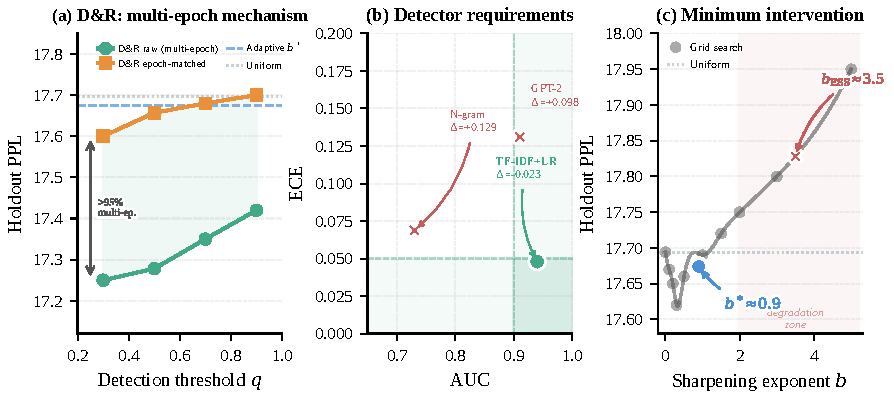
\includegraphics[width=\textwidth]{fig1_overview}
\caption{Three effectiveness conditions for detect-and-reweight.
\textbf{(a)}~D\&R achieves the best raw perplexity (PPL); epoch-matched controls reveal that multi-epoch exposure on filtered data accounts for the bulk of the advantage (\S\ref{sec:results}).
\textbf{(b)}~Only detectors with both high AUC \emph{and} low ECE fall in the effective zone; comparable AUC with poor calibration degrades PPL below uniform.
\textbf{(c)}~Adaptive $\bstar{\approx}0.9$ operates near the grid-search optimum, while ESS-only $b{\approx}3.5$ falls in the degradation zone.}
\label{fig:overview}
\end{figure*}

Despite growing adoption, the paradigm's effectiveness conditions are poorly characterized.
What mechanism drives D\&R's strong performance, and how does it compare to soft reweighting under controlled conditions?
What detector properties are necessary for effective reweighting?
How does the reweighting mechanism behave across contamination levels, and can $b$ be set without per-model grid search?

We investigate these questions through controlled experiments on Qwen3-0.6B continued pretraining (132M FineWeb tokens, $\rho{=}0.4$, 5 seeds), with extensions to $\rho \in \{0.2, 0.6\}$ and 1.7B parameters (\S\ref{sec:limitations} discusses scope).
To ground the analysis of exponent selection, we implement a dual-constrained formulation as an illustrative application: find the minimum $b$ such that $\aeff(b) \geq \tau$ (quality floor, motivated by convergence theory~\citep{wang2026survive}), subject to $\mathrm{ESS}(b) \geq \nmin$ (stability ceiling)~\citep{kish1965survey,vehtari2024psis}.

Our analysis yields three findings:
\begin{itemize}[nosep,leftmargin=*]
\item \textbf{D\&R as the strongest strategy.}
D\&R outperforms all reweighting methods in our setting (PPL $17.250$ vs.\ $17.674$, 3 seeds); epoch-matched controls attribute ${>}$95\% of the advantage to multi-epoch exposure on filtered data, reducing the gap to $\Delta{=}0.017$ (Table~\ref{tab:epoch_match}).

\item \textbf{Detector requirements for effective reweighting.}
Both sufficient discrimination (area under the ROC curve; AUC) and good calibration (expected calibration error; ECE) are empirically observed requirements in our self-contamination setting; a high-AUC but poorly calibrated detector degrades performance below uniform (3 detectors, 3 seeds; \S\ref{sec:robustness}).

\item \textbf{Minimum intervention outperforms maximization.}
An $\aeff$ quality constraint binds in ${\sim}$50\% of batches at ${\approx}4{\times}$ lower sharpening exponents than an ESS-only alternative (\S\ref{sec:regime}); at $\rho{=}0.6$, ESS-only collapses toward uniform while the dual constraint maintains its advantage.
\end{itemize}
To demonstrate the minimum-intervention principle, we derive a dual-constrained adaptive $\bstar$ that eliminates per-model grid search ($\Delta{=}{-}0.023$ at $\rho{=}0.4$, $-$0.032 at $\rho{=}0.6$; Table~\ref{tab:main}), with transferable defaults ($\tau{=}0.7$, $\nmin{=}\lfloor B/2 \rfloor$).
The method fails at $\rho{=}0.2$; at 1.7B it shows no degradation but the benefit diminishes.
